\documentclass{plantillaPPT}
\titulo{8}{Coordenadas Polares}
\begin{document}
\primeraDiapo

\begin{frame}{Área Encerrada por una Curva Polar}
\framesubtitle{Definición}

\begin{definicion}
    El área encerrada bajo una curva polar \(r=f(\theta)\) en el intervalo \(\theta\in[\alpha, \beta]\) está dada por:

\[\frac{1}{2}\int_\alpha^\beta (f(\theta))^2\, d\theta\]

\end{definicion}
\end{frame}

\begin{frame}{Ejemplo Importante}
\centering
\vspace{0.3cm}
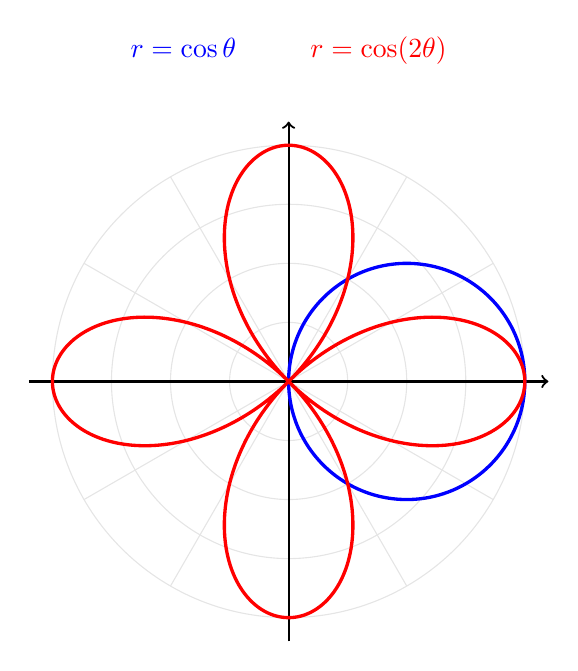
\begin{tikzpicture}[scale=3]

  % Ejes polares sutiles (círculos guía y radios cada 30°)
  \foreach \r in {0.25,0.5,0.75,1}{
    \draw[gray!20, thin] (0,0) circle (\r);
  }
  \foreach \a in {0,30,...,330}{
    \draw[gray!20, thin] (0,0) -- (\a:1);
  }

  % Ejes cartesianos sin etiquetas
  \draw[thick,->] (-1.1,0) -- (1.1,0);
  \draw[thick,->] (0,-1.1) -- (0,1.1);

  % Curva 1: r = cos(θ), suave
  \draw[blue, very thick, smooth, samples=1000, domain=0:360, variable=\t]
    plot ({cos(\t)*cos(\t)}, {cos(\t)*sin(\t)});

  % Curva 2: r = cos(2θ), suave
  \draw[red, very thick, smooth, samples=1000, domain=0:360, variable=\t]
    plot ({cos(2*\t)*cos(\t)}, {cos(2*\t)*sin(\t)});

  % Leyenda centrada arriba
  \node[align=center,font=\bfseries] at (0,1.4)
    {\textcolor{blue}{$r=\cos\theta$} \quad\quad \textcolor{red}{$r=\cos(2\theta)$}};

\end{tikzpicture}
\end{frame}



\begin{frame}{Problema 1}
\framesubtitle{Práctica 8}

1. Sean $C_1$ la lemniscata de ecuación $(x^2+y^2)^2 = (x^2-y^2)$ y $C_2$ el cuadrado de lado 1 y centro $(\frac{1}{2}, \frac{1}{2})$, donde los segmentos de recta $L_1 = \{(x,1):0\leq x \leq1\}$ y $L_2 = \{(1,y):0\leq y\leq1\}$ corresponden a dos de sus lados.

$(a)$ Determine la ecuación polar de $C_1$, $L_1$ y $L_2$. \\
$(b)$ Considerando ambas curvas en el plano polar,, determine los puntos de intersección de $C_1$ con el polo. \\
$(c)$ Escriba la integral que permite calcular el área de la región al exterior de $C_1$ e interior a $C_2$.
    
\end{frame}

\begin{frame}{Problema 1}
\framesubtitle{Práctica 8}
\centering

\includegraphics[width=0.8\textwidth]{C2 2025-2/imagenes/ayud8img2.png}
    
\end{frame}

\begin{frame}{Problema 2}
\framesubtitle{Práctica 8}

2. Sean $C_1$ y $C_2$ dos curvas en coordenadas polares definidas como:
\begin{equation*}
    C_1: r=3\sin(\theta), \quad \theta\in[0,\pi] \quad \text{y} \quad C_2:r=1+\sin(\theta),\quad \theta\in[0,2\pi]
\end{equation*}
$(a)$ Determine la ecuación en coordenadas rectangulares de $C_1$.\\[3pt]
$(b)$ Verifique que los puntos de intersección entre ambas curvas son $P_1(\frac{3}{2}, \frac{\pi}{6})$ y $P_2(\frac{3}{2},\frac{5\pi}{6})$.\\[3pt]
$(c)$ Escriba la integral que permite calcular el área de la región interior a $C_1$ y exterior a $C_2$.
    
\end{frame}

\begin{frame}{Problema 2}
\framesubtitle{Práctica 8}

\centering

\includegraphics[width=0.8\textwidth]{C2 2025-2/imagenes/ayud8img3.png}
    
\end{frame}

\begin{frame}{Problema 3}
\framesubtitle{Práctica 8}
3. La figura adjunta muestra la gráfica polar de la expresión $r = -\cos(\frac{3}{2}\theta)$ para $0\leq\theta\leq2\pi$. Determine una expresión para determinar el área de indicada en la figura, sin desarrollar las integrales.

\begin{center}
    
\includegraphics[width=0.5\textwidth]{C2 2025-2/imagenes/ayud8img.png}
\end{center}
    
\end{frame}

\begin{frame}{Longitud de Arco en Coor. Polares}
\framesubtitle{Definición}

\begin{definicion}
    Sea \(f\) una función para la cual \(f'\) es continua sobre un intervalo \(]\alpha, \beta[\). Entonces la longitud \(L\) de la gráfica \(r=f(\theta)\) sobre el intervalo está dada por:

    \[L(C) = \int_\alpha^\beta \sqrt{r^2+\left(\frac{dr}{d\theta}\right)^2}\, d\theta\]
    
\end{definicion}

\end{frame}
    
\begin{frame}{Problema 4}
\framesubtitle{Práctica 8}

4. Determine la longitud de las siguientes curvas:\\[5pt]
$(a)$ La flor $r = \sin(3\theta)$, con $0\leq\theta\leq\pi$.\\
$(b)$ el espiral $r = e^\theta$, con $\theta\leq0$. \textbf{Indicación: }Utilice la definición de integral impropia.
    
\end{frame}

\end{document}